\section{The solid Chair44 (R44), \texorpdfstring{$\solid$}{Q}}\label{sec:solid}

% ledger: O1, O9, O6, O12 (Figure 3), R1; source proof/PROOFS_registered.md R§1, 1.1; solid/r44_solid.json; Lean solid_mesh_exact
The \emph{carrier} is the seven-cube chair
\[
  \carrier=\bigcup_{a\in\{0,1\}^3,\ a\ne(1,1,1)}\bigl(a+[0,1]^3\bigr),
\]
the $2\times2\times2$ cube with one corner cube removed, of volume $7$. Its boundary consists of
$24$ exposed unit squares, the \emph{panels}: the six outer faces of the $2$-cube contribute
$4+4+4+3+3+3=21$ of them, and the notch left by the missing cube the remaining three. Order the
panels lexicographically by outward normal axis and doubled centre (\cref{fig:carrier}); on each panel use the two
remaining coordinate axes, in increasing order, as tangent coordinates. Relative to the panel's
centre, mark the eight points
\[
  \bigl(\pm\tfrac18,\pm\tfrac14\bigr),\qquad \bigl(\pm\tfrac14,\pm\tfrac18\bigr),
\]
so that all $192$ marks lie in $\tfrac18\Z^3$ and no two coincide. At each mark erect a square
pyramid (\cref{fig:feature}): the base is the axis-parallel square of half-width $\eta=1/100$ centred at the mark, and
the apex is displaced from the panel by $a/10000$ along the outward normal, where $a$ is a nonzero
integer of absolute value between $1$ and $12$ read from a fixed table of $192$ signed entries.
A positive $a$ is a protrusion, a negative $a$ a recess, and the rest of the panel stays flat.
The resulting solid $\solid$ (\cref{fig:tile,fig:panel}) has rational vertex coordinates; it is
defined once, as one unmarked shape, and the indices we use to name its features describe the
construction and impose no rule on how copies may meet. Its volume is exactly $7$: the signed
volumes of the pyramids cancel, because each of the twelve groups of features described below
has as many protrusions as recesses of the same height.

\begin{figure}[ht]
  \centering
  
\includegraphics[width=\linewidth]{print-preview/figure3-corrected.pdf}
  \caption{Oblique and plan views of panel~$13$, the panel outlined in \cref{fig:tile}, with
  the same eight square-pyramid features. Their centres are unchanged; bases are enlarged
  $\times 5$ and signed heights $\times 80$, preserving polarities and relative heights.
  Labels give the signed coefficient $a$: the true height is $a/10000$ and the true base
  side is $1/50$. The panel has outward normal $-y$; the plan view uses global axes $x,z$.}
  \label{fig:panel}
\end{figure}

\begin{figure}[ht]
  \centering
  \resizebox{\linewidth}{!}{% generated by paper/scripts/carrier_panels.py from solid/native_panels.csv
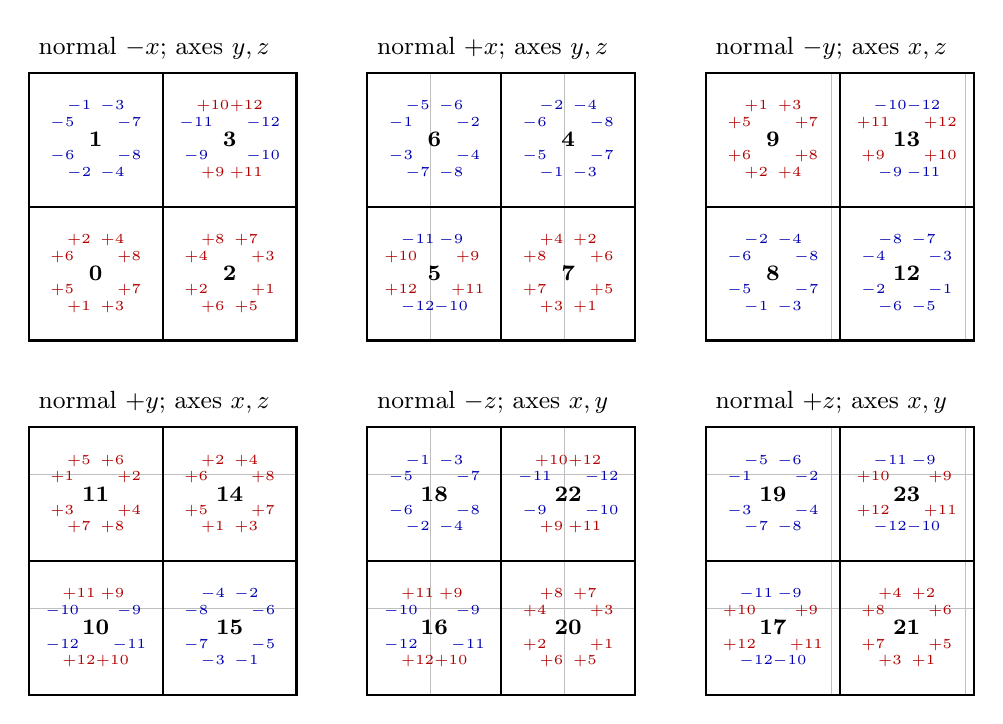
\begin{tikzpicture}[x=1cm,y=1cm,font=\scriptsize]
  \node[anchor=south west,font=\small] at (0.0,3.4499999999999997) {normal $-x$; axes $y,z$};
  \draw[gray!50] (0.0,0.0) grid[step=1.7] (3.4,3.4);
  \draw[thick] (0.0,0.0) rectangle (1.7,1.7);
  \node[font=\footnotesize\bfseries] at (0.85,0.85) {0};
  \node[font=\tiny,text=red!70!black] at (0.6375,0.425) {$+1$};
  \node[font=\tiny,text=red!70!black] at (0.6375,1.275) {$+2$};
  \node[font=\tiny,text=red!70!black] at (1.0625,0.425) {$+3$};
  \node[font=\tiny,text=red!70!black] at (1.0625,1.275) {$+4$};
  \node[font=\tiny,text=red!70!black] at (0.425,0.6375) {$+5$};
  \node[font=\tiny,text=red!70!black] at (0.425,1.0625) {$+6$};
  \node[font=\tiny,text=red!70!black] at (1.275,0.6375) {$+7$};
  \node[font=\tiny,text=red!70!black] at (1.275,1.0625) {$+8$};
  \draw[thick] (0.0,1.7) rectangle (1.7,3.4);
  \node[font=\footnotesize\bfseries] at (0.85,2.55) {1};
  \node[font=\tiny,text=blue!70!black] at (0.6375,2.125) {$-2$};
  \node[font=\tiny,text=blue!70!black] at (0.6375,2.9749999999999996) {$-1$};
  \node[font=\tiny,text=blue!70!black] at (1.0625,2.125) {$-4$};
  \node[font=\tiny,text=blue!70!black] at (1.0625,2.9749999999999996) {$-3$};
  \node[font=\tiny,text=blue!70!black] at (0.425,2.3375) {$-6$};
  \node[font=\tiny,text=blue!70!black] at (0.425,2.7625) {$-5$};
  \node[font=\tiny,text=blue!70!black] at (1.275,2.3375) {$-8$};
  \node[font=\tiny,text=blue!70!black] at (1.275,2.7625) {$-7$};
  \draw[thick] (1.7,0.0) rectangle (3.4,1.7);
  \node[font=\footnotesize\bfseries] at (2.55,0.85) {2};
  \node[font=\tiny,text=red!70!black] at (2.3375,0.425) {$+6$};
  \node[font=\tiny,text=red!70!black] at (2.3375,1.275) {$+8$};
  \node[font=\tiny,text=red!70!black] at (2.7625,0.425) {$+5$};
  \node[font=\tiny,text=red!70!black] at (2.7625,1.275) {$+7$};
  \node[font=\tiny,text=red!70!black] at (2.125,0.6375) {$+2$};
  \node[font=\tiny,text=red!70!black] at (2.125,1.0625) {$+4$};
  \node[font=\tiny,text=red!70!black] at (2.9749999999999996,0.6375) {$+1$};
  \node[font=\tiny,text=red!70!black] at (2.9749999999999996,1.0625) {$+3$};
  \draw[thick] (1.7,1.7) rectangle (3.4,3.4);
  \node[font=\footnotesize\bfseries] at (2.55,2.55) {3};
  \node[font=\tiny,text=red!70!black] at (2.3375,2.125) {$+9$};
  \node[font=\tiny,text=red!70!black] at (2.3375,2.9749999999999996) {$+10$};
  \node[font=\tiny,text=red!70!black] at (2.7625,2.125) {$+11$};
  \node[font=\tiny,text=red!70!black] at (2.7625,2.9749999999999996) {$+12$};
  \node[font=\tiny,text=blue!70!black] at (2.125,2.3375) {$-9$};
  \node[font=\tiny,text=blue!70!black] at (2.125,2.7625) {$-11$};
  \node[font=\tiny,text=blue!70!black] at (2.9749999999999996,2.3375) {$-10$};
  \node[font=\tiny,text=blue!70!black] at (2.9749999999999996,2.7625) {$-12$};
  \node[anchor=south west,font=\small] at (4.3,3.4499999999999997) {normal $+x$; axes $y,z$};
  \draw[gray!50] (4.3,0.0) grid[step=1.7] (7.699999999999999,3.4);
  \draw[thick] (6.0,1.7) rectangle (7.7,3.4);
  \node[font=\footnotesize\bfseries] at (6.85,2.55) {4};
  \node[font=\tiny,text=blue!70!black] at (6.6375,2.125) {$-1$};
  \node[font=\tiny,text=blue!70!black] at (6.6375,2.9749999999999996) {$-2$};
  \node[font=\tiny,text=blue!70!black] at (7.0625,2.125) {$-3$};
  \node[font=\tiny,text=blue!70!black] at (7.0625,2.9749999999999996) {$-4$};
  \node[font=\tiny,text=blue!70!black] at (6.425,2.3375) {$-5$};
  \node[font=\tiny,text=blue!70!black] at (6.425,2.7625) {$-6$};
  \node[font=\tiny,text=blue!70!black] at (7.275,2.3375) {$-7$};
  \node[font=\tiny,text=blue!70!black] at (7.275,2.7625) {$-8$};
  \draw[thick] (4.3,0.0) rectangle (6.0,1.7);
  \node[font=\footnotesize\bfseries] at (5.1499999999999995,0.85) {5};
  \node[font=\tiny,text=blue!70!black] at (4.9375,0.425) {$-12$};
  \node[font=\tiny,text=blue!70!black] at (4.9375,1.275) {$-11$};
  \node[font=\tiny,text=blue!70!black] at (5.3625,0.425) {$-10$};
  \node[font=\tiny,text=blue!70!black] at (5.3625,1.275) {$-9$};
  \node[font=\tiny,text=red!70!black] at (4.725,0.6375) {$+12$};
  \node[font=\tiny,text=red!70!black] at (4.725,1.0625) {$+10$};
  \node[font=\tiny,text=red!70!black] at (5.574999999999999,0.6375) {$+11$};
  \node[font=\tiny,text=red!70!black] at (5.574999999999999,1.0625) {$+9$};
  \draw[thick] (4.3,1.7) rectangle (6.0,3.4);
  \node[font=\footnotesize\bfseries] at (5.1499999999999995,2.55) {6};
  \node[font=\tiny,text=blue!70!black] at (4.9375,2.125) {$-7$};
  \node[font=\tiny,text=blue!70!black] at (4.9375,2.9749999999999996) {$-5$};
  \node[font=\tiny,text=blue!70!black] at (5.3625,2.125) {$-8$};
  \node[font=\tiny,text=blue!70!black] at (5.3625,2.9749999999999996) {$-6$};
  \node[font=\tiny,text=blue!70!black] at (4.725,2.3375) {$-3$};
  \node[font=\tiny,text=blue!70!black] at (4.725,2.7625) {$-1$};
  \node[font=\tiny,text=blue!70!black] at (5.574999999999999,2.3375) {$-4$};
  \node[font=\tiny,text=blue!70!black] at (5.574999999999999,2.7625) {$-2$};
  \draw[thick] (6.0,0.0) rectangle (7.7,1.7);
  \node[font=\footnotesize\bfseries] at (6.85,0.85) {7};
  \node[font=\tiny,text=red!70!black] at (6.6375,0.425) {$+3$};
  \node[font=\tiny,text=red!70!black] at (6.6375,1.275) {$+4$};
  \node[font=\tiny,text=red!70!black] at (7.0625,0.425) {$+1$};
  \node[font=\tiny,text=red!70!black] at (7.0625,1.275) {$+2$};
  \node[font=\tiny,text=red!70!black] at (6.425,0.6375) {$+7$};
  \node[font=\tiny,text=red!70!black] at (6.425,1.0625) {$+8$};
  \node[font=\tiny,text=red!70!black] at (7.275,0.6375) {$+5$};
  \node[font=\tiny,text=red!70!black] at (7.275,1.0625) {$+6$};
  \node[anchor=south west,font=\small] at (8.6,3.4499999999999997) {normal $-y$; axes $x,z$};
  \draw[gray!50] (8.6,0.0) grid[step=1.7] (12.0,3.4);
  \draw[thick] (8.6,0.0) rectangle (10.299999999999999,1.7);
  \node[font=\footnotesize\bfseries] at (9.45,0.85) {8};
  \node[font=\tiny,text=blue!70!black] at (9.237499999999999,0.425) {$-1$};
  \node[font=\tiny,text=blue!70!black] at (9.237499999999999,1.275) {$-2$};
  \node[font=\tiny,text=blue!70!black] at (9.6625,0.425) {$-3$};
  \node[font=\tiny,text=blue!70!black] at (9.6625,1.275) {$-4$};
  \node[font=\tiny,text=blue!70!black] at (9.025,0.6375) {$-5$};
  \node[font=\tiny,text=blue!70!black] at (9.025,1.0625) {$-6$};
  \node[font=\tiny,text=blue!70!black] at (9.875,0.6375) {$-7$};
  \node[font=\tiny,text=blue!70!black] at (9.875,1.0625) {$-8$};
  \draw[thick] (8.6,1.7) rectangle (10.299999999999999,3.4);
  \node[font=\footnotesize\bfseries] at (9.45,2.55) {9};
  \node[font=\tiny,text=red!70!black] at (9.237499999999999,2.125) {$+2$};
  \node[font=\tiny,text=red!70!black] at (9.237499999999999,2.9749999999999996) {$+1$};
  \node[font=\tiny,text=red!70!black] at (9.6625,2.125) {$+4$};
  \node[font=\tiny,text=red!70!black] at (9.6625,2.9749999999999996) {$+3$};
  \node[font=\tiny,text=red!70!black] at (9.025,2.3375) {$+6$};
  \node[font=\tiny,text=red!70!black] at (9.025,2.7625) {$+5$};
  \node[font=\tiny,text=red!70!black] at (9.875,2.3375) {$+8$};
  \node[font=\tiny,text=red!70!black] at (9.875,2.7625) {$+7$};
  \draw[thick] (10.299999999999999,0.0) rectangle (11.999999999999998,1.7);
  \node[font=\footnotesize\bfseries] at (11.149999999999999,0.85) {12};
  \node[font=\tiny,text=blue!70!black] at (10.937499999999998,0.425) {$-6$};
  \node[font=\tiny,text=blue!70!black] at (10.937499999999998,1.275) {$-8$};
  \node[font=\tiny,text=blue!70!black] at (11.362499999999999,0.425) {$-5$};
  \node[font=\tiny,text=blue!70!black] at (11.362499999999999,1.275) {$-7$};
  \node[font=\tiny,text=blue!70!black] at (10.725,0.6375) {$-2$};
  \node[font=\tiny,text=blue!70!black] at (10.725,1.0625) {$-4$};
  \node[font=\tiny,text=blue!70!black] at (11.575,0.6375) {$-1$};
  \node[font=\tiny,text=blue!70!black] at (11.575,1.0625) {$-3$};
  \draw[thick] (10.299999999999999,1.7) rectangle (11.999999999999998,3.4);
  \node[font=\footnotesize\bfseries] at (11.149999999999999,2.55) {13};
  \node[font=\tiny,text=blue!70!black] at (10.937499999999998,2.125) {$-9$};
  \node[font=\tiny,text=blue!70!black] at (10.937499999999998,2.9749999999999996) {$-10$};
  \node[font=\tiny,text=blue!70!black] at (11.362499999999999,2.125) {$-11$};
  \node[font=\tiny,text=blue!70!black] at (11.362499999999999,2.9749999999999996) {$-12$};
  \node[font=\tiny,text=red!70!black] at (10.725,2.3375) {$+9$};
  \node[font=\tiny,text=red!70!black] at (10.725,2.7625) {$+11$};
  \node[font=\tiny,text=red!70!black] at (11.575,2.3375) {$+10$};
  \node[font=\tiny,text=red!70!black] at (11.575,2.7625) {$+12$};
  \node[anchor=south west,font=\small] at (0.0,-1.05) {normal $+y$; axes $x,z$};
  \draw[gray!50] (0.0,-4.5) grid[step=1.7] (3.4,-1.1);
  \draw[thick] (0.0,-4.5) rectangle (1.7,-2.8);
  \node[font=\footnotesize\bfseries] at (0.85,-3.65) {10};
  \node[font=\tiny,text=red!70!black] at (0.6375,-4.075) {$+12$};
  \node[font=\tiny,text=red!70!black] at (0.6375,-3.225) {$+11$};
  \node[font=\tiny,text=red!70!black] at (1.0625,-4.075) {$+10$};
  \node[font=\tiny,text=red!70!black] at (1.0625,-3.225) {$+9$};
  \node[font=\tiny,text=blue!70!black] at (0.425,-3.8625) {$-12$};
  \node[font=\tiny,text=blue!70!black] at (0.425,-3.4375) {$-10$};
  \node[font=\tiny,text=blue!70!black] at (1.275,-3.8625) {$-11$};
  \node[font=\tiny,text=blue!70!black] at (1.275,-3.4375) {$-9$};
  \draw[thick] (0.0,-2.8) rectangle (1.7,-1.0999999999999999);
  \node[font=\footnotesize\bfseries] at (0.85,-1.9499999999999997) {11};
  \node[font=\tiny,text=red!70!black] at (0.6375,-2.375) {$+7$};
  \node[font=\tiny,text=red!70!black] at (0.6375,-1.525) {$+5$};
  \node[font=\tiny,text=red!70!black] at (1.0625,-2.375) {$+8$};
  \node[font=\tiny,text=red!70!black] at (1.0625,-1.525) {$+6$};
  \node[font=\tiny,text=red!70!black] at (0.425,-2.1624999999999996) {$+3$};
  \node[font=\tiny,text=red!70!black] at (0.425,-1.7374999999999998) {$+1$};
  \node[font=\tiny,text=red!70!black] at (1.275,-2.1624999999999996) {$+4$};
  \node[font=\tiny,text=red!70!black] at (1.275,-1.7374999999999998) {$+2$};
  \draw[thick] (1.7,-2.8) rectangle (3.4,-1.0999999999999999);
  \node[font=\footnotesize\bfseries] at (2.55,-1.9499999999999997) {14};
  \node[font=\tiny,text=red!70!black] at (2.3375,-2.375) {$+1$};
  \node[font=\tiny,text=red!70!black] at (2.3375,-1.525) {$+2$};
  \node[font=\tiny,text=red!70!black] at (2.7625,-2.375) {$+3$};
  \node[font=\tiny,text=red!70!black] at (2.7625,-1.525) {$+4$};
  \node[font=\tiny,text=red!70!black] at (2.125,-2.1624999999999996) {$+5$};
  \node[font=\tiny,text=red!70!black] at (2.125,-1.7374999999999998) {$+6$};
  \node[font=\tiny,text=red!70!black] at (2.9749999999999996,-2.1624999999999996) {$+7$};
  \node[font=\tiny,text=red!70!black] at (2.9749999999999996,-1.7374999999999998) {$+8$};
  \draw[thick] (1.7,-4.5) rectangle (3.4,-2.8);
  \node[font=\footnotesize\bfseries] at (2.55,-3.65) {15};
  \node[font=\tiny,text=blue!70!black] at (2.3375,-4.075) {$-3$};
  \node[font=\tiny,text=blue!70!black] at (2.3375,-3.225) {$-4$};
  \node[font=\tiny,text=blue!70!black] at (2.7625,-4.075) {$-1$};
  \node[font=\tiny,text=blue!70!black] at (2.7625,-3.225) {$-2$};
  \node[font=\tiny,text=blue!70!black] at (2.125,-3.8625) {$-7$};
  \node[font=\tiny,text=blue!70!black] at (2.125,-3.4375) {$-8$};
  \node[font=\tiny,text=blue!70!black] at (2.9749999999999996,-3.8625) {$-5$};
  \node[font=\tiny,text=blue!70!black] at (2.9749999999999996,-3.4375) {$-6$};
  \node[anchor=south west,font=\small] at (4.3,-1.05) {normal $-z$; axes $x,y$};
  \draw[gray!50] (4.3,-4.5) grid[step=1.7] (7.699999999999999,-1.1);
  \draw[thick] (4.3,-4.5) rectangle (6.0,-2.8);
  \node[font=\footnotesize\bfseries] at (5.1499999999999995,-3.65) {16};
  \node[font=\tiny,text=red!70!black] at (4.9375,-4.075) {$+12$};
  \node[font=\tiny,text=red!70!black] at (4.9375,-3.225) {$+11$};
  \node[font=\tiny,text=red!70!black] at (5.3625,-4.075) {$+10$};
  \node[font=\tiny,text=red!70!black] at (5.3625,-3.225) {$+9$};
  \node[font=\tiny,text=blue!70!black] at (4.725,-3.8625) {$-12$};
  \node[font=\tiny,text=blue!70!black] at (4.725,-3.4375) {$-10$};
  \node[font=\tiny,text=blue!70!black] at (5.574999999999999,-3.8625) {$-11$};
  \node[font=\tiny,text=blue!70!black] at (5.574999999999999,-3.4375) {$-9$};
  \draw[thick] (4.3,-2.8) rectangle (6.0,-1.0999999999999999);
  \node[font=\footnotesize\bfseries] at (5.1499999999999995,-1.9499999999999997) {18};
  \node[font=\tiny,text=blue!70!black] at (4.9375,-2.375) {$-2$};
  \node[font=\tiny,text=blue!70!black] at (4.9375,-1.525) {$-1$};
  \node[font=\tiny,text=blue!70!black] at (5.3625,-2.375) {$-4$};
  \node[font=\tiny,text=blue!70!black] at (5.3625,-1.525) {$-3$};
  \node[font=\tiny,text=blue!70!black] at (4.725,-2.1624999999999996) {$-6$};
  \node[font=\tiny,text=blue!70!black] at (4.725,-1.7374999999999998) {$-5$};
  \node[font=\tiny,text=blue!70!black] at (5.574999999999999,-2.1624999999999996) {$-8$};
  \node[font=\tiny,text=blue!70!black] at (5.574999999999999,-1.7374999999999998) {$-7$};
  \draw[thick] (6.0,-4.5) rectangle (7.7,-2.8);
  \node[font=\footnotesize\bfseries] at (6.85,-3.65) {20};
  \node[font=\tiny,text=red!70!black] at (6.6375,-4.075) {$+6$};
  \node[font=\tiny,text=red!70!black] at (6.6375,-3.225) {$+8$};
  \node[font=\tiny,text=red!70!black] at (7.0625,-4.075) {$+5$};
  \node[font=\tiny,text=red!70!black] at (7.0625,-3.225) {$+7$};
  \node[font=\tiny,text=red!70!black] at (6.425,-3.8625) {$+2$};
  \node[font=\tiny,text=red!70!black] at (6.425,-3.4375) {$+4$};
  \node[font=\tiny,text=red!70!black] at (7.275,-3.8625) {$+1$};
  \node[font=\tiny,text=red!70!black] at (7.275,-3.4375) {$+3$};
  \draw[thick] (6.0,-2.8) rectangle (7.7,-1.0999999999999999);
  \node[font=\footnotesize\bfseries] at (6.85,-1.9499999999999997) {22};
  \node[font=\tiny,text=red!70!black] at (6.6375,-2.375) {$+9$};
  \node[font=\tiny,text=red!70!black] at (6.6375,-1.525) {$+10$};
  \node[font=\tiny,text=red!70!black] at (7.0625,-2.375) {$+11$};
  \node[font=\tiny,text=red!70!black] at (7.0625,-1.525) {$+12$};
  \node[font=\tiny,text=blue!70!black] at (6.425,-2.1624999999999996) {$-9$};
  \node[font=\tiny,text=blue!70!black] at (6.425,-1.7374999999999998) {$-11$};
  \node[font=\tiny,text=blue!70!black] at (7.275,-2.1624999999999996) {$-10$};
  \node[font=\tiny,text=blue!70!black] at (7.275,-1.7374999999999998) {$-12$};
  \node[anchor=south west,font=\small] at (8.6,-1.05) {normal $+z$; axes $x,y$};
  \draw[gray!50] (8.6,-4.5) grid[step=1.7] (12.0,-1.1);
  \draw[thick] (8.6,-4.5) rectangle (10.299999999999999,-2.8);
  \node[font=\footnotesize\bfseries] at (9.45,-3.65) {17};
  \node[font=\tiny,text=blue!70!black] at (9.237499999999999,-4.075) {$-12$};
  \node[font=\tiny,text=blue!70!black] at (9.237499999999999,-3.225) {$-11$};
  \node[font=\tiny,text=blue!70!black] at (9.6625,-4.075) {$-10$};
  \node[font=\tiny,text=blue!70!black] at (9.6625,-3.225) {$-9$};
  \node[font=\tiny,text=red!70!black] at (9.025,-3.8625) {$+12$};
  \node[font=\tiny,text=red!70!black] at (9.025,-3.4375) {$+10$};
  \node[font=\tiny,text=red!70!black] at (9.875,-3.8625) {$+11$};
  \node[font=\tiny,text=red!70!black] at (9.875,-3.4375) {$+9$};
  \draw[thick] (8.6,-2.8) rectangle (10.299999999999999,-1.0999999999999999);
  \node[font=\footnotesize\bfseries] at (9.45,-1.9499999999999997) {19};
  \node[font=\tiny,text=blue!70!black] at (9.237499999999999,-2.375) {$-7$};
  \node[font=\tiny,text=blue!70!black] at (9.237499999999999,-1.525) {$-5$};
  \node[font=\tiny,text=blue!70!black] at (9.6625,-2.375) {$-8$};
  \node[font=\tiny,text=blue!70!black] at (9.6625,-1.525) {$-6$};
  \node[font=\tiny,text=blue!70!black] at (9.025,-2.1624999999999996) {$-3$};
  \node[font=\tiny,text=blue!70!black] at (9.025,-1.7374999999999998) {$-1$};
  \node[font=\tiny,text=blue!70!black] at (9.875,-2.1624999999999996) {$-4$};
  \node[font=\tiny,text=blue!70!black] at (9.875,-1.7374999999999998) {$-2$};
  \draw[thick] (10.299999999999999,-4.5) rectangle (11.999999999999998,-2.8);
  \node[font=\footnotesize\bfseries] at (11.149999999999999,-3.65) {21};
  \node[font=\tiny,text=red!70!black] at (10.937499999999998,-4.075) {$+3$};
  \node[font=\tiny,text=red!70!black] at (10.937499999999998,-3.225) {$+4$};
  \node[font=\tiny,text=red!70!black] at (11.362499999999999,-4.075) {$+1$};
  \node[font=\tiny,text=red!70!black] at (11.362499999999999,-3.225) {$+2$};
  \node[font=\tiny,text=red!70!black] at (10.725,-3.8625) {$+7$};
  \node[font=\tiny,text=red!70!black] at (10.725,-3.4375) {$+8$};
  \node[font=\tiny,text=red!70!black] at (11.575,-3.8625) {$+5$};
  \node[font=\tiny,text=red!70!black] at (11.575,-3.4375) {$+6$};
  \draw[thick] (10.299999999999999,-2.8) rectangle (11.999999999999998,-1.0999999999999999);
  \node[font=\footnotesize\bfseries] at (11.149999999999999,-1.9499999999999997) {23};
  \node[font=\tiny,text=blue!70!black] at (10.937499999999998,-2.375) {$-12$};
  \node[font=\tiny,text=blue!70!black] at (10.937499999999998,-1.525) {$-11$};
  \node[font=\tiny,text=blue!70!black] at (11.362499999999999,-2.375) {$-10$};
  \node[font=\tiny,text=blue!70!black] at (11.362499999999999,-1.525) {$-9$};
  \node[font=\tiny,text=red!70!black] at (10.725,-2.1624999999999996) {$+12$};
  \node[font=\tiny,text=red!70!black] at (10.725,-1.7374999999999998) {$+10$};
  \node[font=\tiny,text=red!70!black] at (11.575,-2.1624999999999996) {$+11$};
  \node[font=\tiny,text=red!70!black] at (11.575,-1.7374999999999998) {$+9$};
\end{tikzpicture}
}
  \caption{The carrier $\carrier$ and its $24$ panels, numbered as in the text, with the sign
  pattern of the feature heights.}
  \label{fig:carrier}
\end{figure}

% ledger: R1; Lean contact_closure_30, profile_canonical
The table of heights is not arbitrary; it is determined by the substitution of
\cref{sec:substitution} and can be reconstructed from it. Start with the $21$ face contacts that
occur inside the eight-child dissection of the doubled chair and propagate them through
refinement until the set of contacts is closed; it closes at $30$. At every pair of marks that
these contacts bring into coincidence impose that the two heights be opposite, $a_u=-a_v$. This
gives $372$ distinct equations whose signed graph on the $192$ marks has exactly twelve balanced
connected components, each with eight positive and eight negative vertices. Assign the magnitude
$j$ to the $j$-th component in order of its smallest mark, take that mark positive, and transport
signs along the graph. The result is the table of $192$ entries in the solid file, and the twelve
magnitudes $1,\dots,12$ are the twelve components. Because every component uses a distinct
magnitude, two features fit face to face only if they have the same magnitude and opposite sign.

\begin{figure}[ht]
  \centering
  \resizebox{\linewidth}{!}{% fig_feature_geometry.tex — Fig. 2.3: a feature in cross-section (schematic; heights exaggerated,
% the exact numbers are printed). Used by sec2_solid.tex.
\begin{tikzpicture}[x=1cm,y=1cm,font=\small,>={Latex[length=1.6mm]}]
  % left: pyramid cross-section through the apex, along a tangent axis: base [-eta, eta], apex height h
  \begin{scope}
    \draw[thick] (-3.0,0) -- (3.0,0);
    \node[anchor=north] at (-2.4,-0.05) {panel (flat)};
    \draw[thick,fill=red!12] (-1.4,0) -- (0,1.0) -- (1.4,0) -- cycle;
    \draw[<->] (-1.4,-0.45) -- (1.4,-0.45) node[midway,below] {$2\eta = 1/50$};
    \draw[<->] (1.7,0) -- (1.7,1.0) node[midway,right] {$h = a/10000$};
    \draw[dashed] (0,0) -- (0,1.0);
    \draw (-1.4,0) ++(0.55,0) arc (0:35.5:0.55);
    \node at (-0.55,0.25) {$\alpha_j$};
    \node[anchor=north,align=center,text width=6.4cm] at (0,-1.0)
      {$|a|\in\{1,\dots,12\}$; base edge: dihedral $\pi\pm\alpha_j$, $\tan\alpha_j=t_j=j/100$;\\
       apex ridge: dihedral $\pi\mp\beta_j$, $\cos\beta_j=1/(1+t_j^2)$;\\ all $24$ deviations distinct and $<\pi/4$};
  \end{scope}
  % right: the Lipschitz cone at a point of the feature graph
  \begin{scope}[shift={(7.4,0)}]
    \draw[thick] (-2.0,0) -- (2.0,0);
    \fill[black!8] (0,0) -- (-1.8,-0.22) -- (-1.8,-1.4) -- (1.8,-1.4) -- (1.8,-0.22) -- cycle;
    \draw[thick] (0,0) -- (-1.8,-0.22);
    \draw[thick] (0,0) -- (1.8,-0.22);
    \fill (0,0) circle (1.2pt);
    \node[anchor=south] at (0,0.08) {a point of the feature graph};
    \node[anchor=north,align=center,text width=6.4cm] at (0,-1.5)
      {interior cone $w<-L\|v\|$, $L=3/25$:\\ solid angle $\Omega(L)=2\pi\bigl(1-L/\sqrt{1+L^2}\bigr)>7\pi/4$};
  \end{scope}
\end{tikzpicture}
}
  \caption{Schematic feature geometry, with exaggerated height: a pyramid of height $j/10000$,
  base half-width $1/100$, its deviation angles, and the interior cone with slope bound $L=3/25$
  used in \cref{sec:companions}.}
  \label{fig:feature}
\end{figure}

% ledger: O2, O3, O4; Lean boundary_sphere; verify/boundary_sphere.py; imports Moise, Rourke-Sanderson
The boundary of $\solid$ is a triangulated surface with $2{,}138$ vertices, $6{,}408$ edges and
$4{,}272$ triangles (\cref{tab:mesh}), checked triangle by triangle against the construction
above. Every edge lies in exactly two triangles, the triangle graph is connected, the link of
every vertex is a single cycle, and $V-E+F=2$; these are finite facts, verified in Lean and
independently by a script. Two classical results then apply, and we state them exactly as used:
a connected closed triangulated surface with Euler characteristic $2$ is homeomorphic to the
sphere, since an orientable surface of genus $g$ has $\chi=2-2g$ and a non-orientable one with $k$
crosscaps has $\chi=2-k$; and, by the polyhedral Schoenflies theorem of Alexander, a polyhedral
$2$-sphere in $\R^3$ bounds a piecewise-linear $3$-ball \cite{Moi77,RS72}. Hence $\solid$, the
closure of the bounded domain its boundary mesh bounds, is a closed topological $3$-ball. The same
conclusion follows from the tube construction below, which exhibits an ambient homeomorphism
carrying $\carrier$ to $\solid$.

\begin{table}[ht]
  \centering
  \caption{Mesh facts of $\solid$, computed from the solid file with exact arithmetic and
  cross-checked against its recorded counts; the verified statements are \lean{boundary\_sphere},
  \lean{mesh\_angle\_audit} and \texttt{verify/boundary\_sphere.py} (FIGURES.md, Table 5).}
  \label{tab:mesh}
  % generated by paper/scripts/mesh_table.py; from solid/r44_solid.json, exact arithmetic, cross-checked against its counts
\begin{tabular}{L{0.66\linewidth} r}
\toprule
quantity & value \\
\midrule
vertices $V$ & $2{,}138$ \\
edges $E$ & $6{,}408$ \\
triangles $F$ & $4{,}272$ \\
$V-E+F$ & $2$ \\
volume (exact, divergence formula) & $7$ \\
features (square pyramids) & $192$ \\
feature edges; classes (magnitude, base/ridge, sign) $\times$ edges per class & $1{,}536$; $48\times32$ \\
base half-width $\eta$; height unit & $1/100$; $1/10000$ \\
\bottomrule
\end{tabular}

\end{table}

% ledger: O5, O11, R12; Lean planar_area_carrier_recovery_holds (T1, E5; formal proof by diameter endpoints); carrier_feature_frame_reduction_holds (T1n); no_native_symmetry (T1); paper/scripts/planar_areas.py (T2); external review of the manuscript 2026-09-09, finding m2
$\solid$ has no self-isometry. The argument has three parts, and we say once here at what level
each is verified. First, an isometry $g$ with $g\solid=\solid$ preserves the carrier: the nine
large planar boundary regions of $\solid$, one for each coordinate plane at heights $0$, $1$ and
$2$, carry planar areas $2492/625$, $623/625$ and $1869/625$ respectively (the area-four, notch
area-one and area-three regions less their feature bases; exact values from the mesh,
\file{paper/scripts/planar_areas.py}), each more than $9/10$, whereas all the non-axis pyramid
facets together have area less than $1212/15625<1/4$. So $g$ permutes those nine planes; the
three distinct area types identify the height-$0$, height-$1$ and height-$2$ plane triples, hence
$g$ fixes the origin, the corner $(2,2,2)$ and the notch, and maps $\carrier$ to itself
(the Lean theorem \lean{planar\_area\_carrier\_recovery\_holds}, \tier{T1}, proves the same
statement by a different route: a point in a feature tube is at squared distance at most
$1089/100<12$ from every point of $\solid$, so the diameter pairs of $\solid$ lie in the
undeformed carrier and are its antipodal corner pairs, which $g$ permutes; the six corners
recover the centre and the axes, and the preserved missing corner excludes a reversal; the
planar-area calculation above is the written proof). Second, an isometry that preserves both $\solid$
and the chair has a signed permutation matrix as its linear part (the chair's own symmetry group
is the six coordinate permutations) and must carry the table of feature centres and heights to
itself; this reduction to one of the $48$ signed frames is a Lean theorem using
\lean{native\_decide}. Third, among the $48$ signed frames only the identity preserves the
table of $192$ features (a Lean theorem by kernel \lean{decide}). Consequently the stabilizer of
a tiling's family of placements equals its symmetry group, as noted in \cref{sec:terminology}.

% ledger: O6, O7; Lean native_features_length, native_feature_centers_nodup, deviations_distinct, mesh_angle_audit
The $192$ features play $192$ distinct roles: their centres are distinct points of
$\tfrac18\Z^3$, and the twelve magnitudes give two sequences of twelve deviation angles, at the
base edges and at the apex edges of a pyramid of slope $t_j=j/100$, all $24$ distinct: a
coincidence between the two sequences would force $1+(i/100)^2=(1+(j/100)^2)^2$, that is
$10000\,i^2=20000\,j^2+j^4$, which has no solution with $1\le i,j\le 12$ (a Lean theorem by
kernel \lean{decide}). Every one of the $6{,}408$ mesh edges carries a declared dihedral angle,
flat or orthogonal except at the features; the $1{,}536$ feature edges fall into $48$ classes of
$32$, one class per deviation and sign (\cref{tab:mesh}).

% ledger: A16; Lean per_tube_homeomorphisms_holds, feature_tube_maps_glue_holds, feature_tube_map_carries_carrier_holds (T1n); disjointness and boundary identity T1
Around each feature take the normal tube of half-height $\rho=1/100$ over its base. The map
$(u,z)\mapsto(u,\,z+\chi(z)f(u))$, where $f$ is the signed tent function of the pyramid and
$\chi(z)=\max(0,1-|z|/\rho)$, is strictly increasing in $z$ because $\|f\|_\infty\le 12/10000<\rho$,
equals the identity on the boundary of the tube, and carries the flat base to the pyramid. The
$192$ tubes are pairwise disjoint (the marks on a panel are at least $1/8$ apart in one tangent
coordinate and more than $1/5$ from every panel edge, while the bases are $1/50$ across), so the
maps glue to a homeomorphism of $\R^3$ that is the identity outside the tubes and carries
$\carrier$ onto $\solid$. In particular every unit cube of the chair keeps its core
$[\rho,1-\rho]^3$ inside $\solid$, a fact used in \cref{sec:registration}.

% ledger: T14; source proof/PROOFS_registered.md R§11; form 2303.10798 L80 (Tile(a,b))
Finally, the integer heights are a convenient member of a family. Let the twelve component
heights be real numbers $c_1,\dots,c_{12}$, keep the signs of the graph, and use height
$c_j/10000$. With $t_j=|c_j|/100$, the whole proof goes through unchanged provided every $c_j$ is
nonzero and the magnitudes $|c_j|$ are distinct; $1+t_i^2\ne(1+t_j^2)^2$ for all $i,j$; every
$t_j<1$, every $(1+t_j^2)^2<2$, and $63\max_j t_j^2<1$; and the heights stay below $\rho$ and
$\eta$. These are finitely many strict inequalities satisfied by $c_j=j$ (\cref{tab:family}), so
\cref{thm:full} holds on an open twelve-parameter family of solids with the same architecture.
This is not stability under arbitrary perturbation of the boundary, and we claim none.

\begin{table}[ht]
  \centering
  \caption{The parameter family: the exact open conditions of R\S11 and their values at the
  explicit member $c_j=j$, checked with exact rationals (FIGURES.md, Table 7).}
  \label{tab:family}
  \small
  % generated by paper/scripts/parameter_family_table.py; R\S11 conditions verified at c_j = j with exact rationals
\begin{tabular}{L{0.5\linewidth} L{0.42\linewidth}}
\toprule
condition (R\S11) & at $c_j=j$ \\
\midrule
(1) every $c_j\ne0$, magnitudes $|c_j|$ distinct & $|c_j|=1,\dots,12$, distinct \\
(2) $1+t_i^2\ne(1+t_j^2)^2$ for all $i,j$ ($t_j=|c_j|/100$) & holds; smallest gap $39/390625$ \\
(3) $t_j<1$; $(1+t_j^2)^2<2$; $63\max_j t_j^2<1$ & $\max t_j=3/25$; $(1+t^2)^2=401956/390625$; $63t^2=567/625$ \\
(4) heights $|c_j|/10000$ below $\rho=1/100$ and $\eta=1/100$ & $\max=3/2500$ \\
\bottomrule
\end{tabular}

\end{table}
